%----------------------------------------------------------------------------------------
%	PACKAGES AND OTHER DOCUMENT CONFIGURATIONS
%----------------------------------------------------------------------------------------

\documentclass{article}

\usepackage[english]{babel}
\usepackage[utf8]{inputenc}
\usepackage[hyphens]{url}
\usepackage{hyperref}
\usepackage{caption}
\usepackage{fancyhdr} % Required for custom headers
\usepackage{lastpage} % Required to determine the last page for the footer
\usepackage{extramarks} % Required for headers and footers
\usepackage[usenames,dvipsnames]{color} % Required for custom colors
\usepackage{graphicx} % Required to insert images
\usepackage{movie15}
\usepackage{listings} % Required for insertion of code
\usepackage{courier} % Required for the courier font
\usepackage{lipsum} % Used for inserting dummy 'Lorem ipsum' text into the template

\newcommand{\writer}{Davide Peron}

% Margins
\topmargin=-0.45in
\evensidemargin=0in
\oddsidemargin=0in
\textwidth=6.5in
\textheight=9.0in
\headsep=0.25in

\linespread{1.1} % Line spacing

% Set up the header and footer
\pagestyle{fancy}
\lhead{\writer} % Top left head
\chead{Case: Rhino-1151910} % Top center head
\rhead{\today} % Top right header
\lfoot{Signature: } % Bottom left footer
\cfoot{} % Bottom center footer
\rfoot{Page\ \thepage\ of\ \protect\pageref{LastPage}} % Bottom right footer
\renewcommand\headrulewidth{0.4pt} % Size of the header rule
\renewcommand\footrulewidth{0pt} % Size of the footer rule

\fancypagestyle{plain}{
	\fancyfoot[C]{}
}


\setlength\parindent{0pt} % Removes all indentation from paragraphs

\setcounter{secnumdepth}{0} % Removes default section numbers

%----------------------------------------------------------------------------------------
%	TITLE PAGE
%----------------------------------------------------------------------------------------

\title{
	\textmd{\textbf{EXPERT WITNESS REPORT}}\\
	\vspace{0.3in}
	\textsc{\Large IN RELATION TO}\\
	\vspace{0.3in}
	\textmd{\textbf{ILLEGAL RHINOCEROS IMAGES}}\\
	\vspace{0.7in}
	\textmd{\Large \textbf{BY REQUEST OF: }}
	\textsc{\Large Mr. Gareth Davies}\\
	\vspace{0.1in}
	\textmd{\Large \textbf{NAME OF EXPERT: }}
	\textsc{\Large \writer}\\
	\vspace{0.1in}
	\textmd{\Large \textbf{CASE NAME: }}
	\textsc{\Large Rhino-1151910}
	\date{}
}

%----------------------------------------------------------------------------------------

\begin{document}

\parbox{0.4\textwidth}{
	\normalsize
	\textbf{UK Statues and Guidelines Followed:\\
	Criminal Procedure Rules, r 27.1 (1)\\
	Criminal Justice Act 1967, s. 9\\
	Magistrates’ Court Act 1980, s.5B\\
	ACPO Digital Evidence Guidelines}
}

\vspace{0.5in}

{\let\newpage\relax\maketitle}

\centering
\parbox{0.7\textwidth}{
	This statement (consisting of \protect\pageref{LastPage}
	pages each signed by myself) is true to the best of
	my knowledge and belief and I make it knowing that, if tendered in evidence, I shall
	be liable to prosecution if I have wilfully stated in it anything which I know to be false
	or do not believe to be true.
}

\parbox{0.7\textwidth}{
	\vspace{0.2in}
	Signature: \hspace{2in} Date:
}
%----------------------------------------------------------------------------------------
%	TABLE OF CONTENTS
%----------------------------------------------------------------------------------------

%\setcounter{tocdepth}{1} % Uncomment this line if you don't want subsections listed in the ToC

\newpage
\tableofcontents
\newpage

\section{Curriculum Vitae}

I am \writer ~and I am a student in MSc Telecommunications Engineering in University of Padova. I have a Bachelor Degree in Information Engineering.
I have matured my skills in digital devices and networks analysis during my academic career and now I can analyse in depth some devices like smartphones, hard disks, live computers or computer networks.

\vspace{0.3in}

\begin{tabular}{l l}
	\textbf{Name} & \writer\\
	\textbf{Enrolment Number} & 1151910\\
	\textbf{Institutional E-mail} & davide.peron.2@studenti.unipd.it\\
	\textbf{Occupation} & Student in first year of Telecommunications Engineering
\end{tabular}

\section{Instruction/Objectives}

\subsection{Abstract of the case}

The city of New Orleans passed a law in 2004 making possession of nine or more unique rhinoceros images a serious crime. The network  administrator at the University of New Orleans recently alerted police when some illegal rhino traffic was flagged by his network monitoring software. The suspect is a research student and is the primary user of a University computer. The computer hard drive was missing at the time of the alleged offence.

Police have taken a forensically image of USB flash drive seized from one of the University's computer.
Network administrator has recovered three network traces involve the machine with the missing hard drive.

\subsection{Statement of Instructions}
The police has requested that I \writer ~carry out an investigation on the following evidence items:

\begin{itemize}
	\item \textit{RHINOUSB.dd} USB Image
	\item Three network traces
\end{itemize}

The purpose of this report is to outline the result of the investigation in order to answer to the question \textit{Is there any evidence to show that the suspect did store illegal images on the University computer?}

\section{Received Evidence Items}

For each evidence item received, the correspondent MD5 hash checksum was provided.
This checksum has been recalculated at the end of the investigation to ensure the integrity of evidence items.

The provided MD5 checksums are shown in \autoref{tab:checksum}

\begin{table}[h!]
	\centering
	\begin{tabular}{l|l}
		Evidence Item & MD5 checksum\\
		\hline
		RHINOUSB.dd & 80348c58eec4c328ef1f7709adc56a54\\
		rhino.log & c0d0093eb1664cd7b73f3a5225ae3f30\\
		rhino2.log & cd21eaf4acfb50f71ffff857d7968341\\
		rhino3.log & 7e29f9d67346df25faaf18efcd95fc30
	\end{tabular}
	\caption{Evidence Items's MD5 checksums}
	\label{tab:checksum}
\end{table}

\section{Analysis of the evidence items}
A new case in Autopsy\footnote{Some more information about software used during the investigation, can be found in Appendix 1.} has been created, including in it the evidence items. \autoref{fig:rhino_root} shows the root folder of \textit{RHINOUSB.dd} USB image.
Searching for the keyword \textit{rhino} in Autopsy, I have obtained files that contains this word (as shown in \autoref{fig:rhino_search}). We can see at them one by one.

\begin{minipage}[t]{0.45\textwidth}
	\centering
	\vspace{0.5cm}
	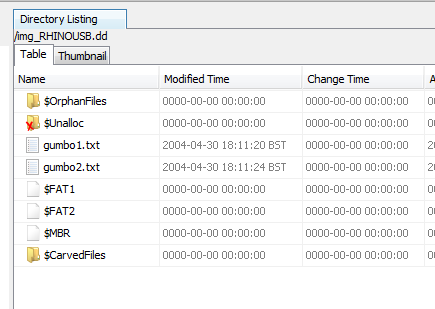
\includegraphics[width=0.9\textwidth]{img/rhinousb_root.png}
	\captionof{figure}{Root folder of \textit{RHINOUSB.dd} image}
	\vspace{1cm}
	\label{fig:rhino_root}
\end{minipage}
\hspace{0.5cm}
\begin{minipage}[t]{0.45\textwidth}
	\centering
	\vspace{0.5cm}
	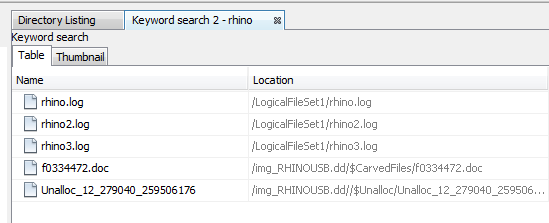
\includegraphics[width=0.9\textwidth]{img/rhino_search.png}
	\captionof{figure}{Result of the search on \textit{RHINOUSB.dd} image}
	\vspace{1cm}
	\label{fig:rhino_search}
\end{minipage}

\subsection{rhino.log analysis}
Opening \textit{rhino.log} I have found that several FTP file transfers have been recorded.
In \textit{rhino.log} has been recorded each FTP command, including the name of the files transferred.
Through this analysis I have found some references to \textit{rhino1.jpg} [\autoref{fig:rhino1}], \textit{rhino3.jpg} [\autoref{fig:rhino3}] and \textit{rhino2.jpg}[\autoref{fig:rhino2}].
This last image was contained into an archive called \textit{contraband.zip}.
In this file I have found also the name of the account from which the crime was performed and the relative password:

\begin{table}[h!]
	\centering
	\begin{tabular}{l|l}
		\textbf{Account} & gnome\\
		\hline
		\textbf{Password} & gnome123\\
	\end{tabular}
	\caption{Data of the account from which the crime was performed}
	\label{tab:account}
\end{table}

\begin{minipage}[h]{0.45\textwidth}
	\centering
	\vspace{0.5cm}
	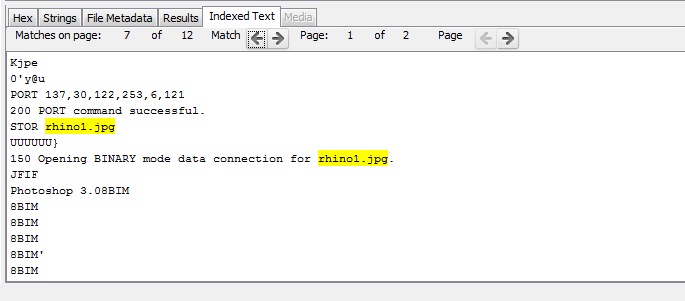
\includegraphics[width=0.9\textwidth]{img/rhino1inrhinolog.png}
	\captionof{figure}{Evidence of existence of \textit{rhino1.jpg} image}
	\vspace{1cm}
	\label{fig:rhino1}
\end{minipage}
\hspace{0.5cm}
\begin{minipage}[h]{0.45\textwidth}
	\centering
	\vspace{0.5cm}
	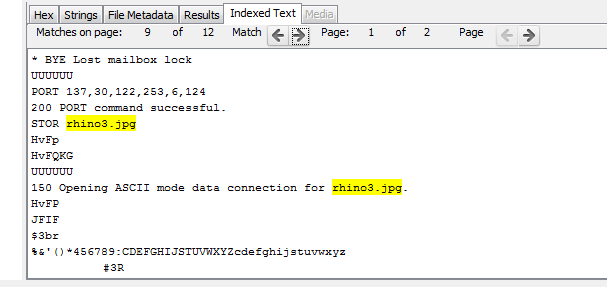
\includegraphics[width=0.9\textwidth]{img/rhino3inrhinolog.png}
	\captionof{figure}{Evidence of existence of \textit{rhino3.jpg} image}
	\vspace{1cm}
	\label{fig:rhino3}
\end{minipage}
\begin{minipage}[h]{0.45\textwidth}
	\centering
	\vspace{0.5cm}
	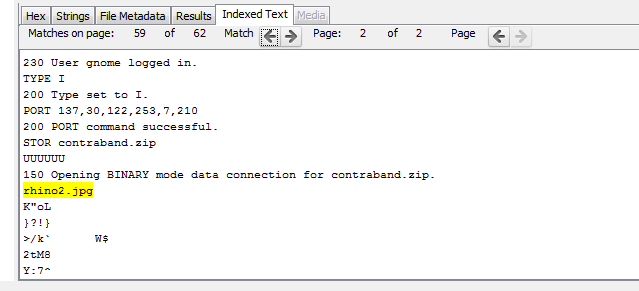
\includegraphics[width=0.9\textwidth]{img/rhino2inrhinolog.png}
	\captionof{figure}{Evidence of existence of \textit{rhino2.jpg} image inside \textit{contraband.zip}}
	\vspace{1cm}
	\label{fig:rhino2}
\end{minipage}

\subsection{rhino2.log analysis}
Opening \textit{rhino2.log} in Autopsy I have found several HTTP Requests.
Between them I have found references to \textit{rhino4.jpg} and \textit{rhino5.gif}, two fraud images (visible in \autoref{fig:rhino45}, \autoref{fig:rhino4} and \autoref{fig:rhino5}).

\begin{figure}[h]
	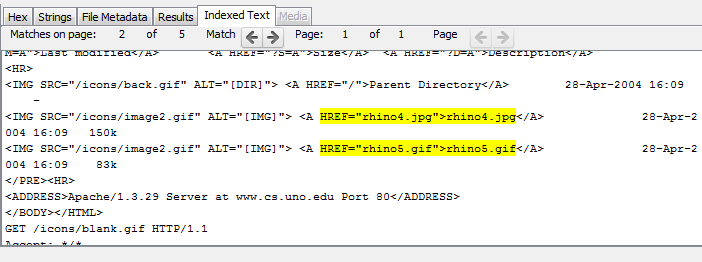
\includegraphics[width=\textwidth]{img/rhino45.png}
	\caption{Evidence of existence of \textit{rhino4.jpg} and \textit{rhino5.gif} images}
	\label{fig:rhino45}
\end{figure}
\begin{minipage}[h]{0.45\textwidth}
	\centering
	\vspace{0.5cm}
	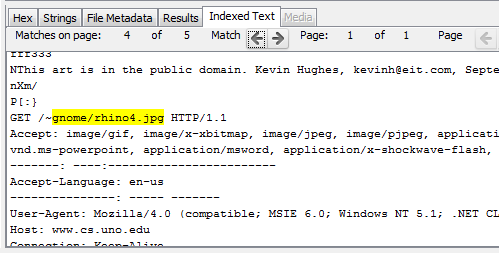
\includegraphics[width=0.9\textwidth]{img/rhino4.png}
	\captionof{figure}{Evidence of existence of \textit{rhino4.jpg} image}
	\vspace{1cm}
	\label{fig:rhino4}
\end{minipage}
\hspace{0.5cm}
\begin{minipage}[h]{0.45\textwidth}
	\centering
	\vspace{0.5cm}
	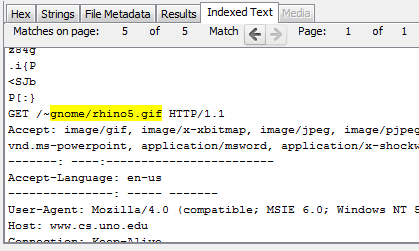
\includegraphics[width=0.9\textwidth]{img/rhino5.png}
	\captionof{figure}{Evidence of existence of \textit{rhino5.gif} image}
	\vspace{1cm}
	\label{fig:rhino5}
\end{minipage}

\subsection{rhino3.log analysis}
Analysing this file, I have found several references to an executable file called \textit{rhino.exe} inside an HTTP Request. One of these references is shown in \autoref{fig:rhinoexe}.

\begin{figure}[h]
	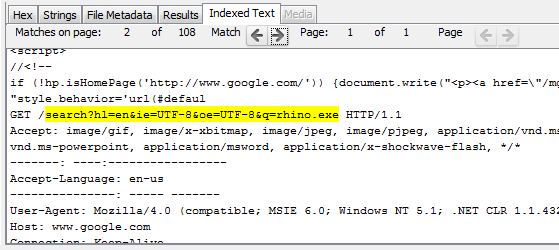
\includegraphics[width=\textwidth]{img/rhinoexe.png}
	\caption{Evidence of existence of \textit{rhino.exe}}
	\label{fig:rhinoexe}
\end{figure}

\subsection{f0334472.doc analysis}
This is a plain text file. Here I have found a brief summary of the crime. In the last part of the text is written the following (proved by \autoref{fig:evtext}):

\vspace{0.5cm}
\parbox{0.8\textwidth}{
	\normalsize
	\textit{Rhino pictures illegal?   Makes me sick.  I “hid” the photos…hehehehe.  Apparently, if there are less than 10 photos, it’s no big deal.\\
	OK.  Things are getting a little weird.  I zapped the hard drive and then threw it into the Mississippi River.  I’m gonna reformat my USB key after this entry, but try not to destroy the good stuff.  I need to change the password on the gnome account that Jeremy gave me.  I can probably just do that at Radio Shack.
	}
}
\vspace{0.5cm}

\begin{figure}[h]
	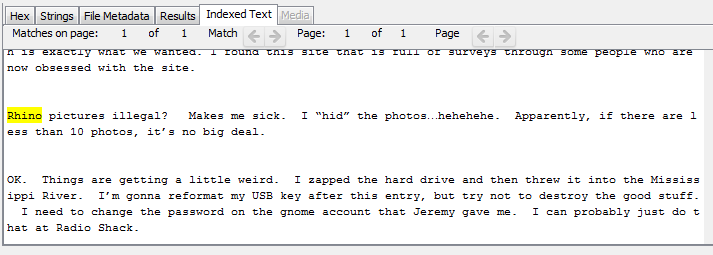
\includegraphics[width=\textwidth]{img/evtext.png}
	\caption{Text found in \textit{f0334472.doc}}
	\label{fig:evtext}
\end{figure}

In this text there is written some information about the USB key used for the crime and about the account from which the crime was performed.
In the metadata of this file I have found some other information about it.

I have found that this text is written with \textit{Microsoft Office Word}.
The metadata of this file also contain the proprietary of the PC from which this text was written, that is \textit{University of New Orleans}.
In the file \textit{Unalloc\_12\_279040\_259506176}, an unallocated part of the memory, there's a longer preamble text after which is appended the same text of \textit{f0334472.doc}.

\subsection{Search for images in img\_RHINOUSB.dd}
Searching in the folders of \textit{img\_RHINOUSB.dd} I have found some rhino's images. They are contained in \textit{\/img\_RHINOUSB.dd\/\$CarvedFiles\/} and are reported in the following.

\begin{minipage}[h]{0.45\textwidth}
	\centering
	\vspace{0.5cm}
	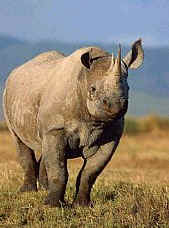
\includegraphics[width=0.9\textwidth]{img/rhino1.jpg}
	\captionof{figure}{Evidence \textit{\/img\_RHINOUSB.dd/\$CarvedFiles/20-f0105848.jpg}}
	\vspace{1cm}
	\label{fig:rhino1img}
\end{minipage}
\hspace{0.5cm}
\begin{minipage}[h]{0.45\textwidth}
	\centering
	\vspace{0.5cm}
	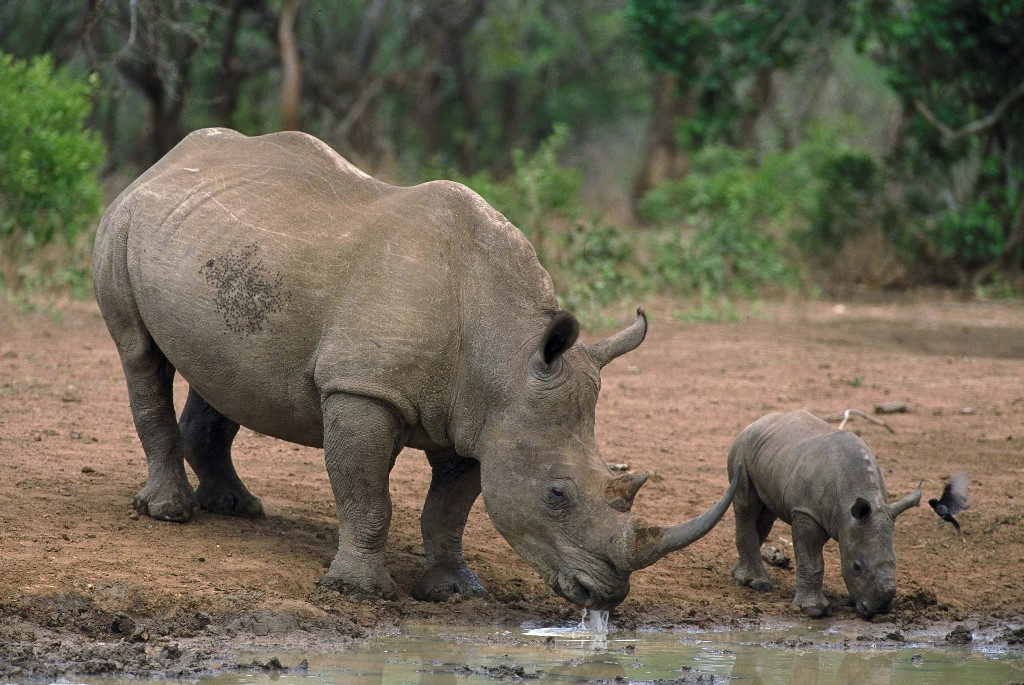
\includegraphics[width=0.9\textwidth]{img/rhino2.jpg}
	\captionof{figure}{Evidence in \textit{\/img\_RHINOUSB.dd/\$CarvedFiles/21-f0105864.jpg}}
	\vspace{1cm}
	\label{fig:rhino2img}
\end{minipage}

\begin{minipage}[h]{0.45\textwidth}
	\centering
	\vspace{0.5cm}
	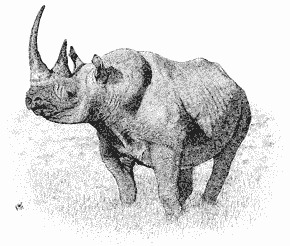
\includegraphics[width=0.9\textwidth]{img/rhino3.jpg}
	\captionof{figure}{Evidence in \textit{\/img\_RHINOUSB.dd/\$CarvedFiles/22-f0106320.gif}}
	\vspace{1cm}
	\label{fig:rhino3img}
\end{minipage}
\hspace{0.5cm}
\begin{minipage}[h]{0.45\textwidth}
	\centering
	\vspace{0.5cm}
	
\includegraphics[width=0.9\textwidth]{img/rhino4.jpg}
	\captionof{figure}{Evidence in \textit{\/img\_RHINOUSB.dd/\$CarvedFiles/23-f0106344.gif}}
	\vspace{1cm}
	\label{fig:rhino4img}
\end{minipage}

\section{Expert Witness Opinion}

During the investigation I have found many evidence of the crime in the evidence items.

The file \textit{f0334472.doc} demonstrate that the accused has hidden rhino pictures inside the USB key. According to this file, this USB key has been reformatted (at \textit{Radio Shack}) hoping not to overwrite the \textit{good} stuff, and the hard drive containing fraud images has been disposed of into the Mississippi River.

This file also hints at a gnome account given to the accused by a certain Jeremy.
This is a connection to \textit{rhino.log}, since a gnome account is used to transfer some fraud images via FTP protocol.
In this file there is also the password of this \textit{gnome} account (that is \textit{gnome123}).

In \textit{rhino.log} and in the other two \textit{.log} files there are several references to fraud images, in specific to \textit{rhino1.jpg}, \textit{rhino2.jpg}, \textit{rhino3.jpg}, \textit{rhino4.jpg} and \textit{rhino5.gif}, and to an \textit{.exe} file, all these are mentioned in FTP or HTTP Requests, this prove that these files have been in the New Orleans University's PC for a while.

Other images have been found in the \textit{\$CarvedFiles/} folder.
In conclusion, I have proved that several rhino's images have been stored in the New Orleans University's PC for a while, I have not recovered these images at all but I have found clear references to them.

\section{Non-Availability of Expert Witness}

\begin{figure}[h]
	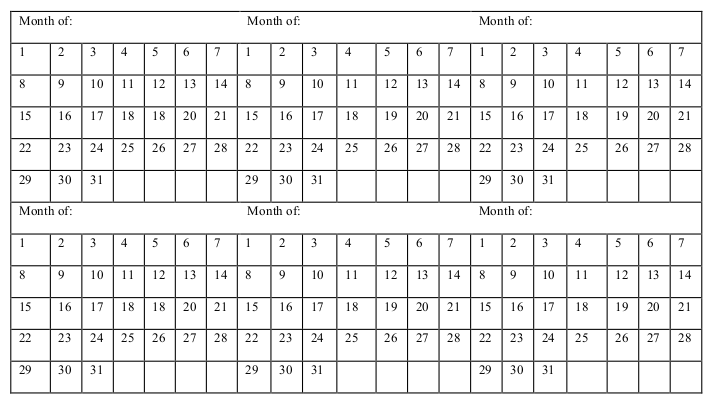
\includegraphics[width=\textwidth]{img/calendar.png}
\end{figure}

\section{Contact Information}

\begin{table}[h!]
	\centering
	\begin{tabular}{l|l}
		\textbf{Full name} & Davide Peron\\
		\hline
		\textbf{Institutional e-mail} & davide.peron.2@studenti.unipd.it\\
		\hline
		\textbf{Work address} & Via Gradenigo 6/b 35131 - Padova Italy\\
	\end{tabular}
	\label{tab:contacts}
\end{table}

\section{Appendix 1 - Software used}

For the whole investigation, I have used Autopsy and S-Tools as Forensics Software Tools and Windows 7 version 6.1 as Operating System.

\subsection{Autopsy}

\begin{table}[h!]
	\centering
	\begin{tabular}{l|l}
		\textbf{Software name} & Autopsy\\
		\hline
		\textbf{Version} & 4.3.0\\
	\end{tabular}
\end{table}

$Autopsy^{TM}$ is an open source digital forensics platform used to examine several types of items, logical or phisical volumes.
It is used by law enforcement, military, and corporate examiners to investigate what happened on a computer. It is based on \textit{The Sleuth Kit}, a collection of open source programs aimed to investigate pieces of software or hardware.

\subsection{S-Tools}

\begin{table}[h!]
	\centering
	\begin{tabular}{l|l}
		\textbf{Software name} & S-Tools\\
		\hline
		\textbf{Version} & 4.00\\
	\end{tabular}
\end{table}

\textit{S-Tools} is an open source software that offer several stenography tools, to create or find files with stenography in them.

I've used this program to ensure that no other rhino images are hidden into some files.


\end{document}
